\documentclass[11pt]{article}

\usepackage{amsmath}
\usepackage{amsthm}

\usepackage{float}
\usepackage{enumitem}
\usepackage{commath}
\usepackage{tikz}
\usetikzlibrary{calc}
\usepackage{cancel}
\usepackage{subfigure}
\usepackage{multicol}

\usepackage{graphicx}
\graphicspath{{images/}}

\usepackage{my_notes}
\usepackage{my_math}

\newenvironment{mybox}
{\begin{tcolorbox}[colback=red!5!white,colframe=red!75!black]}
{\end{tcolorbox}}

%
\theoremstyle{definition}
\newtheorem{theorem}{Theorem}[section]
\newtheorem{definition}[theorem]{Definition}
\newtheorem{corollary}[theorem]{Corollary}

\newenvironment{just}{\textit{Justification.}}{}
\newenvironment{trans}{\textit{Translation.}}{}

\newenvironment{mytbox}
{\begin{tcolorbox}[colback=red!5!white,colframe=red!75!black,title=test]}
{\end{tcolorbox}}

\setlength\parindent{0pt}

\begin{document}
\title{Discrete}
\author{Sean Richardson}
\date{\today}
\maketitle
\tableofcontents

\section{Combinatorics}

Combinatorics studies methods of counting things.

\begin{theorem}[Addition Principle]
    Consider some task $T$. If $T$ can be accomplished by methods $M_1,M_2,\dots,M_n$ which can each be accomplished in $a_1, a_2, \dots, a_n$ ways, then $T$ can be accomplished in $\sum a_k$ ways.
\end{theorem}
\begin{theorem}[Multiplication Principle]
    Consider some task $T$. If $T$ can be broken down into necessary subtasks $t_1,t_2,\dots,t_n$ which can be accomplished in $b_1,b_2,\dots,b_n$ ways, then $T$ can be done in $\prod b_k$ ways.
\end{theorem}
\begin{theorem}
    An arrangement of $n$ objects is called a ``permutation''. There are $n!$ possible permutations.
\end{theorem}
\begin{theorem}
    An arrangement of $r$ objects out of a collection of $n$ objects is called an ``r-permutation''. This can be done in $P(n,r)= {}_{n}P_r = \frac{n!}{(n-r)!}$ ways.
\end{theorem}
\begin{theorem}
    An r-combination is how many combinations of $r$ objects (ignoring order) you can choose from $n$ objects. There are $C(n,r)={}_{n}C_r=(\begin{smallmatrix}n \\ r \end{smallmatrix}) = \frac{n!}{r!(n-r)!}$ ways.
\end{theorem}
\begin{theorem}
    The number of ways to distribute $n$ identical balls into $r$ distinct boxes is $(\begin{smallmatrix} n+r-1 \\ r-1 \end{smallmatrix})$ or $(\begin{smallmatrix} n+r-1 \\ n \end{smallmatrix})$ ways.
\end{theorem}
\begin{proof}
We will now try to determine how many ways $n$ balls can be put in to $r$ boxes. To see this, we use the following trick. Think of balls distributed into boxes in the following structure: $\circ \circ / \circ \circ \circ / \circ / \circ \circ$ where ``$\circ$'' represents balls and the ``/'' symbols divide the balls into categories or boxes. So, the amount of ways to divide $n$ balls into $r$ categories is the amount of ways we can the distribute the dividers among the characters. This is equivalent to ``\textit{characters} choose \textit{dividers}''. There are $n+r-1$ characters and $r-1$ dividers. So, we have $(\begin{smallmatrix} n+r-1 \\ r-1 \end{smallmatrix})$ ways to divide $n$ identical things into $r$ categories. Additionally, we have the following useful equivalency:
\begin{align*}
    \begin{pmatrix} n+r-1 \\ r-1 \end{pmatrix}
    =\frac{(n+r-1)!}{(r-1)!(n+r-1-(r-1))} \\
    =\frac{(n+r-1)!}{(n+r-1-(n))!(n)!}
    = \begin{pmatrix} n+r-1 \\ n \end{pmatrix}
\end{align*}
\end{proof}
\section{Number Theory}
\begin{definition}
    Let $k$ and $n$ be integers with $k \neq 0$. If there exists integer $q$ such that $kq=n$, we say $k$ \emph{divides} $n$, denoted $k \vert n$.
\end{definition}
\begin{theorem}
    Let $a,b,c$ be integers. If $a \vert b$ and $b \vert c$, then $a \vert c$.
\end{theorem}
\begin{theorem}
    Let $a,b,c$ be integers. If $a \vert b$ and $a \vert c$, then $a \vert b+c$.
\end{theorem}
\begin{theorem} [The Division Algorithm]
    Let $m$ and $n$ be integers, with $m>0$. Then, there is a unique pair of integers $q$ and $r$ such that $n = mq+r$ where $0 \leq r < m$. 
\end{theorem}
/*Irrational numbers and $\sqrt{2}$*/
\begin{definition}
    Let $n > 0$ and $p > 1$ be integers. $p$ is \emph{prime} if ``$n\vert p$'' is only true if $n=p$ or $n=1$.
\end{definition}
There is a useful mathematical proof technique called \emph{induction}.
Induction operates in two parts. If you want to prove some statement
involving an arbitrary $n$ is true, you first prove it is true for the
specific case $n=c$ where you choose $c$. Secondly, you show that if the
statement holds for $n=k$, then it holds for $n=k+1$. Then, you are done.
By the first part, you have proved the case $n=c$. Then, combining this
with the second part of the proof, you know it holds for $n=c+1$,$n=c+2$,$n=\dots$ A formal inductive proof has the following form:\\
\underline{Inductive Proof Structure:} \\
    We proceed by the method of Induction, \\
    For the base case of $n=0$, \emph{prove the statement holds for $n=0$} \\
    Now we make the inductive hypothesis that \emph{the statement holds for arbitrary $k$}. \\
    Now we proceed to prove the inductive step \emph{prove that if statement holds for $k$, it holds for $k+1$}. \\
    Thus by induction \emph{the statement holds}. \qed
\section{Logic}
The symbols:
\begin{itemize}
    \item $\lnot$: Represents ``not''. $\lnot A$ is read ``not $A$'' or ``negation of $A$''.
    \item $\land$: Represents ``and''. $A \rightarrow B$ is read ``$A$ and $B$''.
    \item $\lor$: Represents ``or''. $A \lor B$ is read ``$A$ or $B$''.
    \item $\rightarrow$: Represent ``if''. $A \land B$ is read ``$A$ implies $B$'' or ``if $A$ then $B$''.
    \item $\leftrightarrow$: Represent ``necessary and sufficient
        condition''. $A \leftrightarrow B$ is equivalent to $A \rightarrow B$ and $B \rightarrow A$.
    \item $\forall$: The universal quantifier; represents ``for all''. $\forall x \in D$ is read ``for all $x$ in $D$.''
    \item $\exists$: The existential quantifier; represents ``for some'' or ``there exists''. $\exists x \in D$ is read ``there exists an $x$ in $D$''.
    \item $\exists!$: Represent ``there exists unique''. 
\end{itemize}
\begin{definition}
    A statement that is always false called is a \emph{contradiction}. The classic contradiction is $p \land \lnot p$.
\end{definition}
\begin{definition}
    A statement that is always true is called a \emph{tautology}. The classic tautology is $p \lor \lnot p$.
\end{definition}
\begin{theorem}[DeMorgan's Law]~\\
    $\lnot (p \land q) \iff \lnot p \lor \lnot q$ and
    $\lnot (p \lor q) \iff \lnot p \land \lnot q$
\end{theorem}
\begin{theorem}[General DeMorgan's Law]~\\
    $\lnot(p_1 \land p_2 \land \dots \land p_n) \iff (\lnot p_1 \lor \lnot p_2 \lor \dots \lor p_n)$ \\
    $\lnot(p_1 \lor p_2 \lor  \dots \lor  p_n) \iff (\lnot p_1 \land \lnot p_2 \land \dots \land p_n)$ \\
\end{theorem}
\begin{theorem}[Reduction ad absurdum]
    $(p \rightarrow q) \iff ((p \land \lnot q) \rightarrow c)$
\end{theorem}
\begin{theorem}[Modus ponens]
    $((p \leftarrow q) \land p) \implies q$
\end{theorem}
\begin{theorem}[Modus tollens]
    $((p \rightarrow q) \land \lnot q) $
\end{theorem}
\begin{theorem}[Law of syllogism]
    $((p \rightarrow q)\land(q \rightarrow r)) \implies (p \rightarrow r)$
\end{theorem}
\begin{theorem}[Law of disjunctive syllogism]
    $((p \lor q) \land \lnot p) \implies q$
\end{theorem}
\begin{theorem}
    $\lnot(\forall x \in D, p(x)) \iff \exists x \in D, \lnot p(x)$
\end{theorem}
\section{Set Theory}
There exists objects. Objects can be ``in'', ``belong to'' or be
an``element'' of a set. If an object is in a set $S$, we say $a \in S$. If
not, we say $a \notin S$. We can describe the elements of a set $S$ in the
following notation. $S = \{f \vert \text{rule that $f$ must obey} \}$.
\begin{definition}
    Let $A$ and $B$ be sets. If $\forall x \in A, x \in B$ then $A$ is a \emph{subset} of $B$, denoted $A \subseteq B$.
\end{definition}
\begin{definition}
    The set of everything in the relevant universe is denoted $\mathcal{U}$.
\end{definition}
\begin{definition}
    The set with nothing in it is the \emph{empty set}, denoted $\O$. $\O = \{ f \vert f \notin \mathcal{U} \}$.
\end{definition}
\begin{theorem}
For any set $A$, $\O \subseteq A$.
\end{theorem}
\begin{definition}
Let $A$ and $B$ be sets such that $A \subseteq B$ and $B \subseteq A$. Then, we say $A=B$.
\end{definition}
\begin{definition}
Let $A$ and $B$ be sets. If $A \subseteq B$ but $A \neq B$ then $A$ is a \emph{proper subset} of $B$, denoted $A \subset B$.
\end{definition}
\begin{theorem}
The empty set is unique.
\end{theorem}
\begin{definition}
    Let $n$ be a nonnegative integer. A set containing $n$ distinct
    elements is called an \emph{n-set}. 
\end{definition}
\begin{definition}
    Let $A$ be an n-set. $n$ is called the \emph{cardinality} of $A$ or the \emph{order} of $A$, denoted $\vert A \vert = n$
\end{definition}
\begin{definition}
    Let $A$ and $B$ be sets so that $B \in A$ and $\vert B \vert = r$. Then $B$ is said to be an \emph{r-subset} of $A$.
\end{definition}
\begin{theorem}
    There are $(\begin{smallmatrix} n\\r \end{smallmatrix}$). $r$-subsets of and $n$-set.
\end{theorem}
\begin{definition}
    Let $A$ be a set. The set of all subsets of $A$ is called the
    \emph{power set of $A$} denoted $\mathcal{P}(A)$.
\end{definition}
\begin{theorem}
    For any nonnegative integer $n$ there are $2^n$ subsets of an $n$-set $A$. So $\myabs{\mathcal{P}(A)} = 2^n$
    \label{thm:power_combos}
\end{theorem}
/*Note about summing over choose operators*/
\begin{definition}
    Let $A$ and $B$ be sets. The \emph{union} of $A$ and $B$ denoted $A \cup B$ is defined $A \cup B = \{ x \vert x \in A \text{ or } x \in B \}$.
\end{definition}
\begin{definition}
    Let $A$ and $B$ be sets. The \emph{intersection} of $A$ and $B$ denoted $A \cap B$ is defined $A \cap B = \{ x \vert x \in A \text{ and } x \in B \}$.
\end{definition}
\begin{definition}
    Let $A$ and $B$ be sets. If $A \cap B = \O$ then $A$ and $B$ are \emph{disjoint}.
\end{definition}
\begin{theorem}
    Let $A$ and $B$ be sets. Then $\myabs{A \cup B} = \myabs{A} + \myabs{B} - \myabs{A \cap B}$.
\end{theorem}
\begin{theorem} 
    Let $A$ and $B$ be sets \\ Associative laws:\\
    $(A \cup B) \cup C = A \cup (B \cup C)$ and 
    $(A \cap B) \cap C = A \cap (B \cap C)$ \\
    Distributive laws:\\
    $(A \cup B) \cap C = (A \cap C) \cup (B \cap C)$ and
    $(A \cap B) \cap C = (A \cup C) \cap (B \cup C)$
\end{theorem}
\begin{definition}
    Let $A$ and $B$ be sets. The \emph{relative complement} of $B$ \emph{in} $A$, denoted $A \setminus B$ or $A - B$. Its defined as $A \setminus B = \{ x \vert x \in A \text{ and } x \notin B \}$.
\end{definition}
\begin{definition}
    Let $A$ be a set. The \emph{complement} of $A$, denoted $\overline{A}$ is defined as $\overline{A} = \{ x \in \mathcal{U} \vert x \notin A \}$.
\end{definition}
\begin{definition} (DeMorgan's Laws) Let $A$ and $B$ be sets. \\
    Then $\overline{A \cup B} = \overline{A} \cap \overline{B}$ and $\overline{A \cap B} = \overline{A} \cup \overline{B}$
\end{definition}
\section{Pascal and Probability}
\subsection{Pascal's Triangle}
This section is centered around the patterns of Pascal's Triangle and the related theorems. We will define Pascal's Triangle as the following pattern of choose functions:
\begin{figure}[H]
\centering
\begin{subfigure}
    \centering
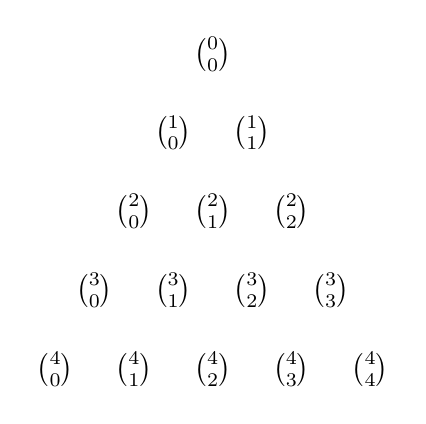
\begin{tikzpicture}
\foreach \n in {0,...,4} {
  \foreach \k in {0,...,\n} {
    \node at (\k-\n/2,-\n) {${\n \choose \k}$};
  }
}
\end{tikzpicture}
\end{subfigure}
\begin{subfigure}
    \centering
\begin{tikzpicture}
    %Row 0
    \def\n{0}; \def\k{0}; \def\val{1};
    \node at (\k-\n/2,-\n) {${\val}$};
    %Row 1
    \def\n{1}; \def\k{0}; \def\val{1};
    \node at (\k-\n/2,-\n) {${\val}$};
    \def\n{1}; \def\k{1}; \def\val{1};
    \node at (\k-\n/2,-\n) {${\val}$};
    %Row 2
    \def\n{2}; \def\k{0}; \def\val{1};
    \node at (\k-\n/2,-\n) {${\val}$};
    \def\n{2}; \def\k{1}; \def\val{2};
    \node at (\k-\n/2,-\n) {${\val}$};
    \def\n{2}; \def\k{2}; \def\val{1};
    \node at (\k-\n/2,-\n) {${\val}$};
    %Row 3
    \def\n{3}; \def\k{0}; \def\val{1};
    \node at (\k-\n/2,-\n) {${\val}$};
    \def\n{3}; \def\k{1}; \def\val{3};
    \node at (\k-\n/2,-\n) {${\val}$};
    \def\n{3}; \def\k{2}; \def\val{3};
    \node at (\k-\n/2,-\n) {${\val}$};
    \def\n{3}; \def\k{3}; \def\val{1};
    \node at (\k-\n/2,-\n) {${\val}$};
    %Row 4
    \def\n{4}; \def\k{0}; \def\val{1};
    \node at (\k-\n/2,-\n) {${\val}$};
    \def\n{4}; \def\k{1}; \def\val{4};
    \node at (\k-\n/2,-\n) {${\val}$};
    \def\n{4}; \def\k{2}; \def\val{6};
    \node at (\k-\n/2,-\n) {${\val}$};
    \def\n{4}; \def\k{3}; \def\val{4};
    \node at (\k-\n/2,-\n) {${\val}$};
    \def\n{4}; \def\k{4}; \def\val{1};
    \node at (\k-\n/2,-\n) {${\val}$};
\end{tikzpicture}
\end{subfigure}
\end{figure}
First, we need some tools to further investigate Pascal's Triangle
\begin{theorem}[Pascal's Identity] Each entry in Pascal's Triangle is exactly equal to the sum of the entry up and to the right along with the entry up and to the left. This is due to the following equality,
    $
        \begin{pmatrix} n \\ k \end{pmatrix}
        +\begin{pmatrix} n \\ k+1 \end{pmatrix}
        =\begin{pmatrix} n+1 \\ k+1 \end{pmatrix}
    $
\end{theorem}
\begin{proof}
    The quantity $(\begin{smallmatrix} n+1 \\ k+1 \end{smallmatrix})$ represents the number of ways to make committees of size $k+1$ from $n+1$ people including you. Each committee either includes you or doesn't. $(\begin{smallmatrix} n \\ k \end{smallmatrix})$ include you and $(\begin{smallmatrix} n \\ k+1 \end{smallmatrix})$ do not. Therefore, the equality holds.
\end{proof}
\begin{theorem}
Each entry in Pascal's Triangle describes precisely how many paths there is
from the top of Pascal's Triangle there is to that entry.
\end{theorem}
\begin{proof}
/*Add inductive proof*/
\end{proof}
\begin{theorem}[The Biomial Theorem]
    The $n$th row of Pascal's Triangle perfectly describes the coefficients of $(x+y)^n$. Or, 
    \begin{equation*}
        (x+y)^n = \sum_{k=0}^n
        \begin{pmatrix} n \\ k \end{pmatrix}x^{n-k}y^k
    \end{equation*}
\end{theorem}
\begin{proof}[Proof 1]
We proceed by induction on $n$,\\
We have the base case of $(x+y)^0 = 1 = \begin{pmatrix} 0 \\ 0 \end{pmatrix}x^0y^0$\\
We make the inductive hypothesis that for some $m \geq 0$,\\ 
\begin{equation*}
(x+y)^m = \sum_{k=0}^m \begin{pmatrix} m \\ k \end{pmatrix}x^{m-k}y^k
\end{equation*}
We will now make the inductive step in showing that 
\begin{equation*}
    (x+y)^{m+1} = \sum_{k=0}^{m+1} \begin{pmatrix} m+1 \\ k \end{pmatrix}x^{(m+1)-k}y^k
\end{equation*}
We begin,
\begin{align*}
    &(x+y)^{m+1}=(x+y)(x+y)^m
    =(x+y)\sum_{k=0}^m \begin{pmatrix}m\\k\end{pmatrix} x^{m-k}y^k\\
    &=\sum_{k=0}^m  \begin{pmatrix}m\\k\end{pmatrix} x^{(m+1)-k}y^k
    +\sum_{k=0}^m \begin{pmatrix}m\\k\end{pmatrix} x^{m-k}y^{k+1}\\
    &\text{Make a change of variables to right sum}\\
    &=\sum_{k=0}^m  \begin{pmatrix}m\\k\end{pmatrix} x^{(m+1)-k}y^k
    +\sum_{k=1}^m+1 \begin{pmatrix}m\\k-1\end{pmatrix} x^{(m+1)-k}y^{k}\\
    &\text{Apply Pascal's Identity}\\
    &=\begin{pmatrix}m\\0\end{pmatrix}x^{m+1}
    +\sum_{k=1}^m \begin{pmatrix} m+1\\k \end{pmatrix}x^{(m+1)-k}y^k
    +\begin{pmatrix}m+1\\m+1\end{pmatrix}y^{m+1}\\
    &=\sum_{k=0}^{m+1} \begin{pmatrix} m+1\\k \end{pmatrix} x^{(m+1)-k} y^k
\end{align*}


We have shown our inductive step and thus conclude our proof by induction.\\
\end{proof}
\begin{proof}[Proof 2] A more intuitive proof of the Binomial Theorem.\\
    Consider ${(x+y)}^n=(x+y)(x+y)\cdots(x+y)$ Multiplying this out is of
    the form $(xx\cdots xx) + (xx\cdots xy) + \cdots + (yy \cdots yy)$
    iterating through all orderings of $x$'s and $y$'s. Every ordering with
    $k$ amount of $y$'s contributes $1$ to the $x^{n-k}y^k$ coefficient.
    There are $(\begin{smallmatrix} n \\ k \end{smallmatrix})$ ways to
    contribute to $x^{n-k}y^k$ terms, so the coefficient of this term is $(\begin{smallmatrix} n \\ k \end{smallmatrix})$. It follows that the full expansion is 
        $(x+y)^n = \sum_{k=0}^n
        (\begin{smallmatrix} n \\ k \end{smallmatrix})x^{n-k}y^k$. Proving the Binomial Theorem.
\begin{corollary}
The case $x=y=1$ in the binomial theorem shows
\begin{equation*}
    \sum\limits_{j=0}^n \begin{pmatrix} n \\ j \end{pmatrix}=2^n
\end{equation*}
\end{corollary}
And the case of $x=-1$, $y=1$ in the binomial theorem shows that
\begin{corollary}
And the case of $x=-1$, $y=1$ in the binomial theorem shows that
\begin{equation*}
\sum\limits_{j=0}^n (-1)^j \begin{pmatrix} n \\ j \end{pmatrix}=0
\end{equation*}
\end{corollary}
\end{proof}
    \marginpar{Add Intuitive proof}
\begin{theorem}
    The sum of some diagonal down and to the right on Pascal's Triangle is described by the term down and to the left of the lowest term in the diagonal. Or, 
    \begin{equation*}
        \begin{pmatrix} k    \\ 0 \end{pmatrix} +
        \begin{pmatrix} k+1  \\ 1 \end{pmatrix} +
        \begin{pmatrix} k+2  \\ 2 \end{pmatrix} +
        \cdots +
        \begin{pmatrix} k+r  \\ r \end{pmatrix} =
        \begin{pmatrix} k+r+1\\ r\end{pmatrix}
    \end{equation*}
    \marginpar{Add Figure}
\end{theorem}
\begin{proof}
    /*Do this, (inductive)*/
\end{proof}
/*After stuff*/
\begin{definition}
    We define the notation $$\begin{pmatrix} n \\ a_1,a_2,\cdots,a_k \end{pmatrix}=\frac{n}{a_1! a_2! \ldots a_k!}$$
\end{definition}
\begin{theorem} [The Multinomial Theorem] For $n \geq 0 \in Z$,
    \begin{equation*}
        {(x_1+x_2+\cdots+x_k)}^{n}=\sum_{\substack{a_1,a_2,\cdots,a_k \geq 0 \\ a_1+a_2+\cdots+a_k=n}}
        \begin{pmatrix} n \\ a_1,a_2,\cdots,a_k \end{pmatrix}
        x_1^{a_1} + x_2^{a_2} + \cdots x_k^{a_k}
    \end{equation*}
\end{theorem}
\begin{proof}
    Consider ${(x_1+x_2+\cdots +x_k)}^n$, which expands to the sum of every ordering of $x_1$'s, $x_2$'s, \ldots, $x_k$'s. The amount of orderings that contribute to an arbitrary $x_1^{a_1} + x_2^{a_2} + \cdots x_k^{a_k}$ is $(\begin{smallmatrix} n!\\a_1! \end{smallmatrix})(\begin{smallmatrix} (n-a_1)!\\a_2 \end{smallmatrix})(\begin{smallmatrix} n-(a_1+\cdots+a_{k-1})\\a_k \end{smallmatrix}) = (\begin{smallmatrix} n \\ a_1,a_2,\cdots,a_k \end{smallmatrix})$. It then follows that, \\
        ${(x_1+x_2+\cdots+x_k)}^{n}=\sum_{\substack{a_1,a_2,\cdots,a_k \geq 0 \\ a_1+a_2+\cdots+a_k=n}}
        \begin{smallmatrix} n \\ a_1,a_2,\cdots,a_k \end{smallmatrix}
        x_1^{a_1} + x_2^{a_2} + \cdots x_k^{a_k}$ which proves the Multinomial Theorem.
\end{proof}
\subsection{Probability}
\begin{definition}
    An \emph{experiment} is an action whose result is one of a finite number of equally likely outcomes.
\end{definition}
\begin{definition}
    The set of outcomes of an experiment is called the \emph{sample space} of the experiment, denoted $S$.
\end{definition}
\begin{definition}
    An \emph{event} is a subspace of the sample space.
\end{definition}
\begin{definition}
    Let $E$ be an event in $S$. Then, the \emph{probability} of $E$ is $P(E)=\frac{\myabs{E}}{\myabs{S}}$.
\end{definition} 
\section{}
\subsection{Relations}
\begin{definition}
    Let $A$ and $B$ be sets. The \emph{Cartesian product} or the \emph{cross product} of $A$ and $B$, is defined $A \times B = \{(a,b) \mid a\in A \text{ and } b\in B \}$.
\end{definition}
\marginpar{multiplication table}
\begin{definition}
    Let $A$ and $B$ be sets. A subset of $A \times B$ is a \emph{relation} from $A$ to $B$
    \label{def:relation}
\end{definition}
\begin{theorem}
    Let $A$ and $B$ be finite sets. $\abs{A\times B} = \abs{A}\abs{B}$.
\end{theorem}
\begin{just}
    The set $A \times B$ is created in a matrix of $(a,b)$ pairs. The matrix is $\abs{A}$ by $\abs{B}$, so it has $\abs{A}\abs{B}$ elements.
\end{just}
\begin{theorem}
    Let $A$ and $B$ be finite sets. The number of relations from $A$ to $B$ is $2^{\abs{A}\abs{B}}$.
\end{theorem}
\begin{proof}
    Let $A$ and $B$ be sets. By Definition~\ref{def:relation}, a relation is a subset any $A \times B$. The number of relations is the number of ways to create a relation, which is the number of subsets of $A \times B$. By Theorem~\ref{thm:power_combos}, this is equivalent to $2^{\abs{A \times B}}=2^{\abs{A}\abs{B}}$.
\end{proof}
\begin{definition}
    Let $R$ be a relation from $A$ to $B$. Then the set $R^{-1}=\{(b,a) \mid (a,b)\in R \}$ is the \emph{inverse relation} of $R$.
\end{definition}
\begin{definition}
    Let $A$ be a set. A subset $R$ of $A \times A$ is a \emph{(binary) relation} on $A$. If $(a,b)\in R$, we say $aRb$, read ``a is related to b''.
\end{definition}
\begin{definition}
    Let $R$ be a relation on $A$. If $aRa$ for $\forall a \in A$, $R$ is \emph{reflexive}.
\end{definition}
\begin{definition}
    Let $R$ be a relation on $A$. If $aRb$ implies $bRa$, $R$ is \emph{symmetric}.
\end{definition}
\begin{definition}
    Let $R$ be a relation on $A$. $R$ is \emph{transitive} if $aRb$ and $bRc$ implies $aRc$.
\end{definition}
\begin{definition}
Let $R$ be a relation on $A$. If $R$ is reflexive, symmetric, and transitive, then $R$ is said to be an \emph{equivalence relation}.
\end{definition}
There will end up being some number of ``bags'' containing elements that are related within a relation.
\marginpar{bags figure}
\begin{definition}
    Let $R$ be an equivalence relation on a set $A$. Let $a\in A$. The set $R_a = \{ x \in A \mid aRx\}$ is called the \emph{equivalence class} of $a$.
\end{definition}
\begin{theorem}
Let $R$ be an equivalence relation on $A$ and let $a,b \in A$. Then either $R_a=R_b$ or $R_a \cap R_b = \O$.
\end{theorem}
\begin{just}
If an equivalence relation represents a bunch of ``bags''. This is saying that an element cannot be in two bags. If an element were in to bags, the transitivity would imply that the bags are actually the same or they are not bags that define equivalence relations.
\end{just}
\begin{definition}
    Let $A$ be a nonempty set. We define $P = \{ A_1,A_2,\dots,A_n \}$, where each $A_i \subseteq A, A_i \neq \O$ for $1 \leq i \leq n$, $A_i \cap A_j = \O$ for $i \neq j$, and $A_1 \cup A_2 \cup \dots A_n = A$. Then, $P$ is a \emph{partition} of $A$.
\end{definition}
\begin{trans}
    A \emph{partition} splits all elements of something into smaller pieces.
\end{trans}
\begin{theorem}
    Let $P = \{ A_1, A_2, \dots, A_n \}$ be a partition on the set $A$. If we define a relation $R$ on $A$ by $aRb$ iff $(a \in A_i) \leftrightarrow (b \in A_i)$ for some $i$, then $R$ is an equivalence relation. 
\end{theorem}
\begin{trans}
    The pieces a partition splits a set $A$ into can describe the ``bags'' of an equivalence relation.
\end{trans}
\begin{proof}
We will show the relation $R$ is reflexive, symmetric, transitive.
\begin{itemize}
    \item Consider an arbitrary $a \in A$. Assume $\lnot aRa$. This implies $\lnot(a \in A_i \leftrightarrow a \in A_i) \Rightarrow (a \in A) \land (a \notin A)$, a contradiction. So, we conclude $aRa$. Because $a$ is arbitrary, we have $\forall a \in A, aRa$. And we have thus concluded reflexivity.
    \item Assume $aRb$. This implies $(a \in A_i) \leftrightarrow (b \in
        A_i) \Rightarrow (b \in A_i) \leftrightarrow (a \in A_i)
        \Rightarrow bRa$. So, we conclude $aRb \rightarrow bRa$, confirming
        symmetry.
    \item Assume $aRb \land aRc$. This implies $(a \in A_i \leftrightarrow b \in A_i) \land (a \in A_i \leftrightarrow c \in A_i) \Rightarrow a \in A_i \leftrightarrow c \in A_i \Rightarrow aRc$, confirming transitivity.
\end{itemize}
$R$ is reflexive, symmetric, and transitive. So, $R$ is an equivalence relation.
\end{proof}
\subsection{Functions}
\begin{definition}[Function]
Let $F$ be a relation from a set $A$ to a set $B$. If each first coordinate appears exactly once in the set of ordered pairs, then $F$ is a \emph{function} from $A$ to $B$.
\end{definition}
\marginpar{show mapping of $F$ from every element of one set to some of
other set}
A function $F$ that maps each element in $A$ to a corresponding element in
$B$ is often notated by $F: A \rightarrow B$.
\begin{theorem}
    Let $A$ and $B$ be finite sets. There are $\myabs{B}^{\myabs{A}}$
    functions from $A$ to $B$.
\end{theorem}
\begin{definition}[Domain and Range]
    Let $F$ be a function from a set $A$ to a set $B$. The set of all first
    coordinates of ordered pairs in $F$ is the \emph{domain} of $F$. ($A$
    is the domain). The set of all second coordinate ordered pairs in $F$
    is called the \emph{range}. The set $B$ is the \emph{codomain} of $F$.
    If $F(a) = b$, we say $b$ is the \emph{image} of $a$ under $F$ and $a$
    is the \emph{pre-image} of $b$.
\end{definition}
\begin{definition}[one-to-one]
Let $A$ and $B$ be sets and $F: A \to B$ a function. If $\forall x_1,x_2
\in A$ we have $x_1 \neq x_2 \implies F(x_1) \neq F(x_2)$, then $F$ is a
\emph{one-to-one} function or an \emph{injection}.
\end{definition}
\begin{theorem}
    Let $A$ and $B$ be finite sets. There are
    $\frac{\myabs{B}!}{(\mymag{B}-\mymag{A})!}$ one-to-one functions from
    $A$ to $B$.
\end{theorem}
\begin{definition}[Onto function]
Let $A$ and $B$ be sets and $f: A \to B$ a function. If $\forall b \in B,
\exists a\in A$ such that $f(a) = b$, then $f$ is an \emph{onto} function
or a \emph{surjection}.
\end{definition}
\begin{definition}[Bijection]
Let $A$ and $B$ be sets and $f: A \to B$ a function. If $f$ is 1-1 and
onto, $f$ is a \emph{bijection}. If a bijection exists from $A$ to $B$, we
say there is a \emph{one-to-one correspondence} between $A$ and $B$.
\end{definition}
\begin{definition}[Cardinality]
    If there exists a bijection $f: \{1,2,\dots,n\} \to A$ then we say the
    \emph{cardinality} of $A$ is $n$, denoted $\myabs{A}=n$.
\end{definition}
\begin{definition}[Composition]
    Let $F: A \to B$ and $G: B \to C$. Then the \emph{composition} of $G$
    with $F$, denoted $G \circ F: A \to C$ is a function defined by
    $$ G \circ F: a \mapsto G(F(a)) \ \ \forall a \in A$$
\end{definition}
\begin{definition}[The Pigeonhole Principle]
    Let $A$ be an $n$-set and $B$ an $m$-set with $n > m$. Then $f: A \to
    B$ cannot be 1--1.
\end{definition}
\end{document}
